\section*{Umsetzung} % (fold)
\label{sec:umsetzung}

%% Hier schreiben wie wir das netz gebaut haben


Tabelle \ref{tab:zeiten} zeigt die von uns approximierten Zeiten für die vorhandenen Transitionen. Für alle Handlungen wird davon ausgegangen das die für die Handlung notwendigen Zutaten und Materialien dem Koch direkt vorliegen und der Koch sofort mit dem Vorgang beginnen kann.

\begin{table}[ht]
\centering
\caption{Zeiten für Handlungen/Transitionen}
\vspace{4mm}
\label{tab:zeiten}

	\begin{tabularx}{\textwidth}{| >{\setlength\hsize{\hsize}\centering}X | >{\setlength\hsize{\hsize}\centering}X |}
	\hline
	Handlung / Transition & Zeit in s \tabularnewline \hline \hline
	Vanilleschote aufschneiden & 	3 + Dist.negexp(1) \tabularnewline \hline
    Mark aufkochen & 	180 + Dist.negexp(5) \tabularnewline \hline
    Milch \& Stärke verrühren & 	5 + Dist.negexp(4) \tabularnewline \hline
    Zitrone \& Wein mischen &  5 + Dist.negexp(1) \tabularnewline \hline
    Weinsoße schaumig rühren &  40 + Dist.negexp(5) \tabularnewline \hline
    Milch/Stärke \& Vanillemilch verrühren &  5 + Dist.negexp(1) \tabularnewline \hline
    Vanillecreme aufkochen & 60 + Dist.negexp(10) \tabularnewline \hline
    Vanillecreme abkühlen lassen & 260 + Dist.negexp(40) \tabularnewline \hline
    Ei trennen &  5 + Dist.negexp(1) \tabularnewline \hline
    Eiweiss schlagen &  20 + Dist.negexp(4) \tabularnewline \hline
    Schnee unter Vanillecreme unterheben &  5 + Dist.negexp(5) \tabularnewline \hline
    Vanillecreme + Schnee abfüllen &  2 + Dist.negexp(2) \tabularnewline \hline
    Vanillecreme mit heißer Weinsoße auffüllen &  2 + Dist.negexp(2) \tabularnewline \hline

    \end{tabularx}
\end{table}
Das erweiterte Petrinetz sieht wie in Abbildung \ref{pic:petrinetz} dargestellt aus. Es wurde ein \textit{Hilfs-Platz} namens Tasse hinzugefügt, der dazu dient, dass die Stärke nicht doppelt für die Herstellung von dem Milch-Stärke-Gemisch verwendet wird, und das System verklemmt. Zusätzlich wurde ein Platz namens \textit{Koch} hinzugefügt, der eine Kante zu allen Transitionen die eine Tätigkeit eines Kochs repräsentieren hat. An diesem Platz wird die Anzahl der Köche durch die Startmarkierung verändert.
\begin{figure}[ht]
  \fbox{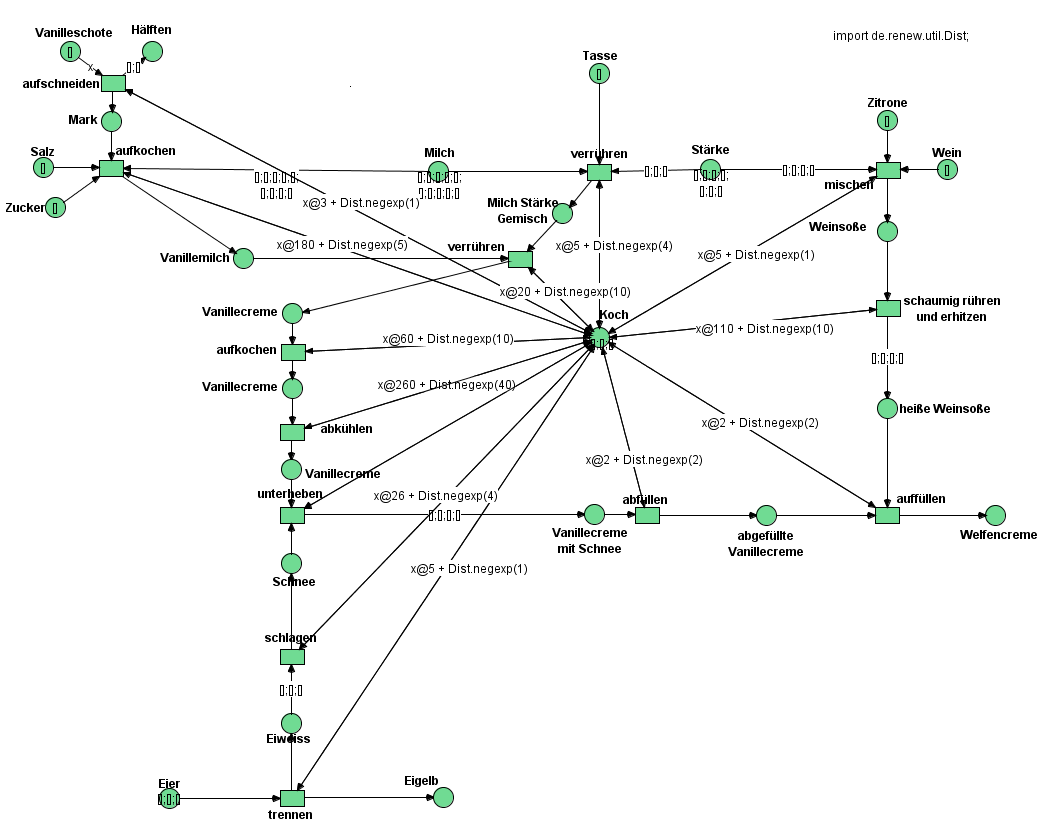
\includegraphics[width=1\textwidth]{pics/net.png}}
  \caption{Das auf Basis der Rezeptur erstellte Petrinetz, erweitert zum timed Net}
  \label{pic:petrinetz}
\end{figure}

Die Durchführung haben wir mithilfe eines von uns geschriebenen Autohotkey-Skripts automatisiert, worüber das Starten und Stoppen getriggert wurde. Die Datenausgabe haben wir über den Start von Renew über den folgenden Aufruf in eine Textdatei schreiben lassen:
\begin{lstlisting}
java -jar loader.jar gui > data.txt
\end{lstlisting}

% section aufgabe_3 (end)
